\documentclass[10pt,twocolumn]{article}
\usepackage{geometry}
\geometry{verbose,headsep=3cm,tmargin=2.5cm,bmargin=2.5cm,lmargin=2.0cm,rmargin=2.0cm}
\usepackage{graphicx}
\usepackage{xcolor}
\usepackage[font=small]{caption}
\usepackage{amsmath,amssymb,latexsym}
\usepackage{marvosym}
\usepackage{url}
\usepackage{lipsum}
\usepackage{bm}
\usepackage{float}
\usepackage[english]{babel}
\usepackage{hyperref}
\usepackage{subcaption}
\usepackage{subfloat}
\usepackage{epsf}
\usepackage{float}
\usepackage{mathpazo}
\usepackage{pifont}
\usepackage{wrapfig}
\usepackage{multicol}
\usepackage{enumitem}
\usepackage{xcolor}
\usepackage{framed}
\usepackage[utf8]{inputenc}
\graphicspath{{plots/}}
\usepackage{framed}
\usepackage{textcomp}
\usepackage{braket}
\newcommand{\highlight}[1]{%
  \colorbox{orange!50}{$\displaystyle#1$}}
% Default fixed font does not support bold face
\DeclareFixedFont{\ttb}{T1}{txtt}{bx}{n}{10} % for bold
\DeclareFixedFont{\ttm}{T1}{txtt}{m}{n}{10}  % for normal

% Custom colors
\usepackage{color}
\definecolor{deepblue}{rgb}{0,0,0.5}
\definecolor{deepred}{rgb}{0.6,0,0}
\definecolor{deepgreen}{rgb}{0,0.5,0}

\usepackage{listings}

% Python style for highlighting
\newcommand\pythonstyle{\lstset{
language=Python,
basicstyle=\ttm,
otherkeywords={self},             % Add keywords here
keywordstyle=\ttb\color{deepblue},
emph={MyClass,__init__},          % Custom highlighting
emphstyle=\ttb\color{deepred},    % Custom highlighting style
stringstyle=\color{deepgreen},
frame=tb,                         % Any extra options here
showstringspaces=false            % 
}}


% Python environment
\lstnewenvironment{python}[1][]
{
\pythonstyle
\lstset{#1}
}
{}

% Python for external files
\newcommand\pythonexternal[2][]{{
\pythonstyle
\lstinputlisting[#1]{#2}}}

% Python for inline
\newcommand\pythoninline[1]{{\pythonstyle\lstinline!#1!}}
% Document font:
\usepackage{charter}


\begin{document}

%%% HEADER --------------------------------------------------------------
% ------------------------------------------------------------------------

\twocolumn[{
\begin{@twocolumnfalse}

  \begin{center}
%\textcolor{lgray}
    \vskip-5em

    \hfill
    \fontsize{10}{10}\selectfont {\textit{Bruxelles, June 2020}}
    \vskip2ex
	\vspace{5ex}
    \fontsize{20}{10}\selectfont {The tensor necessity}
      \vspace{1ex}
      
      \fontsize{16}{10}\selectfont {-- a short story about momentum transport in fluids}
  \noindent%
    
\vskip1ex

{\rule{\textwidth}{0.5pt}}

  \end{center}
  
    \fontsize{7}{10}\selectfont {This work is licensed under the Creative Commons Attribution-NonCommercial-ShareAlike 4.0 International (CC BY-NC-SA 4.0) license.}

\vspace{6mm}

\end{@twocolumnfalse}
}]

%%% HEADER END -----------------------------------------------------------
% ------------------------------------------------------------------------

\vspace{10mm}

\setlength{\parindent}{0cm}

\fontsize{14}{10}\selectfont {Kamila Zdybał}

\vspace{2mm}

\fontsize{8}{10}\selectfont {\textit{Université libre de Bruxelles, kamila.zdybal@ulb.ac.be}}

\fontsize{8}{10}\selectfont {\textit{kamilazdybal.github.io/science-docs, kamila.zdybal@gmail.com}}

\section*{Preface}

\setlength{\parindent}{1em}
\setlength{\parskip}{0.5em}

At first encounter, tensors can seem like strange mathematical objects. It can be challenging to grasp their meaning and their relevance might not be immediately obvious. At the same time, tensors are indispensable when studying fluid dynamics. So what's with the tensors and why do we need them?

In this document we would like to convince you that we necessarily need tensors in fluid dynamics! We will motivate their usefulness using a simple example of a Couette flow. Hopefully by the end of this document you will find tensors very useful mathematical objects that make our life easier. Join me on the journey!

Please feel free to contact me with any suggestions, corrections or comments.

\section*{Keywords}

\textit{tensor, momentum transport, transport phenomena, fluid dynamics, Couette flow}

%\tableofcontents

\section*{Viscous momentum flux tensor}

To build our intuition around tensor quantities we will begin our journey with an illustrative example. We will look at the momentum transport in the Couette flow -- the flow of fluid between two parallel plates. The top plate is stationary and the bottom plate moves in the positive $x$-direction with the velocity $\mathbf{u}$, as presented in Figure~\ref{fig:couette-flow}.

Suppose that we start with an initial situation when both plates are stationary. At some moment in time, we begin moving the bottom plate, reaching the velocity $\mathbf{u}$ after a while. You may already expect that the moment we started moving the bottom plate something interesting starts to happen to the fluid in-between -- it begins moving as well. As the flow develops, the moving plate successively "drags" fluid particles in the layer directly above that plate. Once those fluid particles are set in motion in the positive $x$-direction, that moving layer of fluid "drags" another layer directly on top of it. This "dragging" progresses upward in the positive $y$-direction, until at the top stationary plate the fluid is stagnant again. After a sufficient amount of time, the fluid motion becomes steady. In the steady state, the velocity profile between two plates is fully developed and does not change in time anymore. The steady state velocity profile in the Couette flow is a linear function of $y$ (this is plotted as well in Figure~\ref{fig:couette-flow}). This is something that we will not prove here but you can give it a try as an exercise!
\begin{figure}[H]
\centering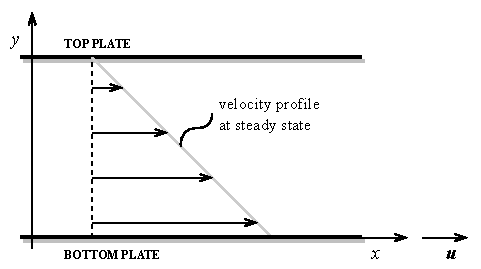
\includegraphics[width=7cm]{couette-flow.pdf}
\caption{The Couette flow is the flow of fluid between two parallel plates.}
\label{fig:couette-flow}
\end{figure}

\begin{wrapfigure}{R}{0.1\textwidth}
\centering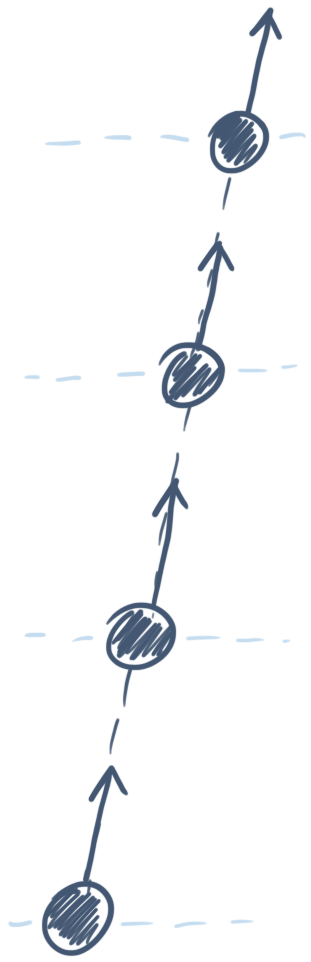
\includegraphics[width=1.8cm]{molecular-collisions.png}
\label{fig:molecular-collisions}
\end{wrapfigure}
If we assume that the fluid flow between the two plates is laminar we may assume that the fluid flows in thin layers, or \textit{laminates}, stacked one on top of the other. Knowing the velocity profile, we know exactly what the velocity of each laminate is. Since we know $\mathbf{u}(y)$, we can compute that velocity at any position $y$. In the flow described in Figure~\ref{fig:couette-flow}, the laminate at the lower $y$-coordinate will have a larger velocity than the laminate at the larger $y$-coordinate. This holds in our case where we assumed that the bottom plate is moving and the fluid velocity decreases to zero once we reach the top plate. In Figure~\ref{fig:momentum-transport-in-laminates}, we have drawn three such laminates, each having a thickness $dy$. Similar reasoning can be done assuming that the top plate is moving with the velocity $\mathbf{u}$, and the bottom plate is stationary.

Knowing the velocities, we also know the momentum carried by each laminate. We will in fact consider the specific momentum -- the momentum per unit volume -- for the purpose of this discussion. Let's look at the situation from the perspective of one of the laminates whose $y$-coordinate is simply denoted $y$. This laminate is marked in gray in Figure~\ref{fig:momentum-transport-in-laminates}. Its specific momentum is $\rho \mathbf{u}|_{y}$.  It gains momentum from the faster moving laminate directly below it, whose specific momentum is $\rho \mathbf{u}|_{y-dy}$. It also looses momentum to the slower laminate directly above it, whose specific momentum is $\rho \mathbf{u}|_{y+dy}$. Such transport of momentum is in practice possible due to molecular collisions. Every collision is an opportunity to exchange momentum. When molecules from one laminate collide with molecules from another laminate, momentum can be transported in the positive $y$-direction. The "dragging", that we talked about before, is thus achieved by the momentum transport. The faster moving laminate gives some of its momentum to the slower moving one.

%Note that this can only happen in the world with friction! Since in fluids friction is accounted for by viscosity it becomes clear that viscosity plays a role in transporting momentum\footnote{Although in a "frictionless world" momentum can still be transported by a fluid but not by means of viscosity. We will move to other forms of momentum transport in the next section.}.
\begin{figure}[H]
\centering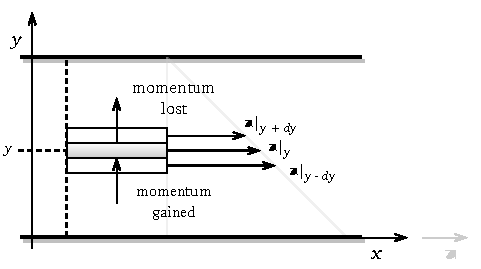
\includegraphics[width=7cm]{momentum-transport-in-laminates.pdf}
\caption{Transporting momentum between the fluid \textit{laminates} from the perspective of one of the laminates (marked in gray).}
\label{fig:momentum-transport-in-laminates}
\end{figure}
\begin{figure}[H]
\centering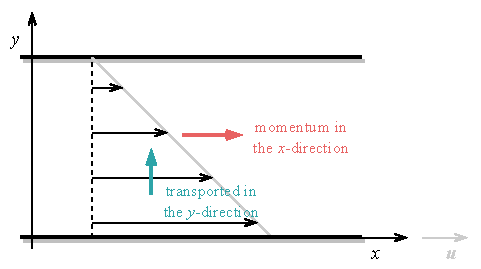
\includegraphics[width=7cm]{couette-flow-momentum-transport.pdf}
\caption{In the Couette flow, the momentum in the $x$ direction is transported in the $y$ direction. The transported momentum is called the \textit{momentum flux}.}
\label{fig:couette-flow-momentum-transport}
\end{figure}
An important concept now emerges. Momentum is a vector quantity that has a direction of the velocity vector. In our example of the Couette flow, momentum of every laminate has the direction parallel to the $x$-axis (in accordance with the velocity profile). However, the transport of that momentum is happening in the direction parallel to the $y$-axis: from the laminates at the lower $y$-coordinate to the laminates at the larger $y$-coordinate. This is conceptually presented in Figure~\ref{fig:couette-flow-momentum-transport}. 

\begin{wrapfigure}{L}{0.2\textwidth}
\centering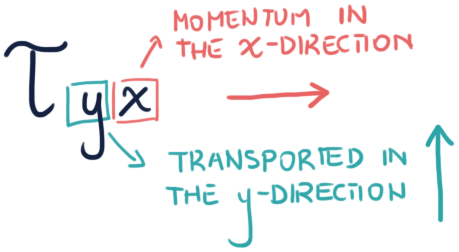
\includegraphics[width=3cm]{tau_y_x.png}
\label{fig:tau_y_x}
\end{wrapfigure}
The transported momentum (also called the \textit{momentum flux}) is denoted with a symbol $\tau_{yx}$. Notice now that this quantity, $\tau_{yx}$, carries information about two directions. The first one, telling us which direction is the momentum vector pointing. The second one, telling us which direction that momentum is being transported.

Tensors are objects that allow us to associate more than one direction to a physical quantity. In the case of the Couette flow considered here, the tensor quantity $\tau$ representing the momentum flux, would be called a \textit{second-order tensor} because it carries information about two directions. Tensors can also be thought of as a generalization of the concept of a vector. A vector is characterized by the magnitude and one direction -- it is thus a \textit{first-order tensor}. In general, tensors can be characterized by the magnitude and one or multiple directions attached to it. Of course, we need to create such notation that we know what each direction means physically. In our example, one direction was keeping track of the transport and the other was keeping track of the direction of the velocity vector. Hopefully, by now you can appreciate that tensors are very useful tools in fluid dynamics, where vector quantities (such as momentum) can be transported in many directions!

If we considered a different system than the Couette flow, perhaps there would be momentum in the $x$-direction transported in the $z$-direction. Or, momentum in the $y$-direction transported in the $x$-direction\footnote{Can you think of a real situation when momentum in the $x$-direction is transported in the $x$-direction?}.

In a three-dimensional world, the momentum vector can be pointing in any of the three directions $x$, $y$ or $z$, and can be transported in any of the three directions $x$, $y$ or $z$. Tensors allow us to keep track of all those directions as well. If we wanted to account for all these possibilities in three-dimensions we would need $3 \times 3 = 9$ quantities $\tau_{ij}$. For convenience, we often write out the elements of a tensor in a form of a table that resembles a matrix. Unlike in a scalar matrix, this table has additional information attached to every element -- the directions represented. Those directions are agreed upon and often we can omit specifying them and just write out the magnitudes in a form of a matrix. But we should keep in mind that the directions are still there, even if at the "backstage" of the matrix.

Figure \ref{fig:tensor-in-matrix-form} shows an example of the most general second-order tensor that could represent viscous momentum flux in a three-dimensional fluid flow. We noted the directions that each element is keeping track of. Once we write down a specific $\tau_{ij}$, its directions can be understood through the indices $i$ and $j$. In the case of a Couette flow we needed only one of those elements - $\tau_{yx}$ - since there was only one direction for momentum and only one direction in which that momentum was transported.

\begin{figure}[H]
\centering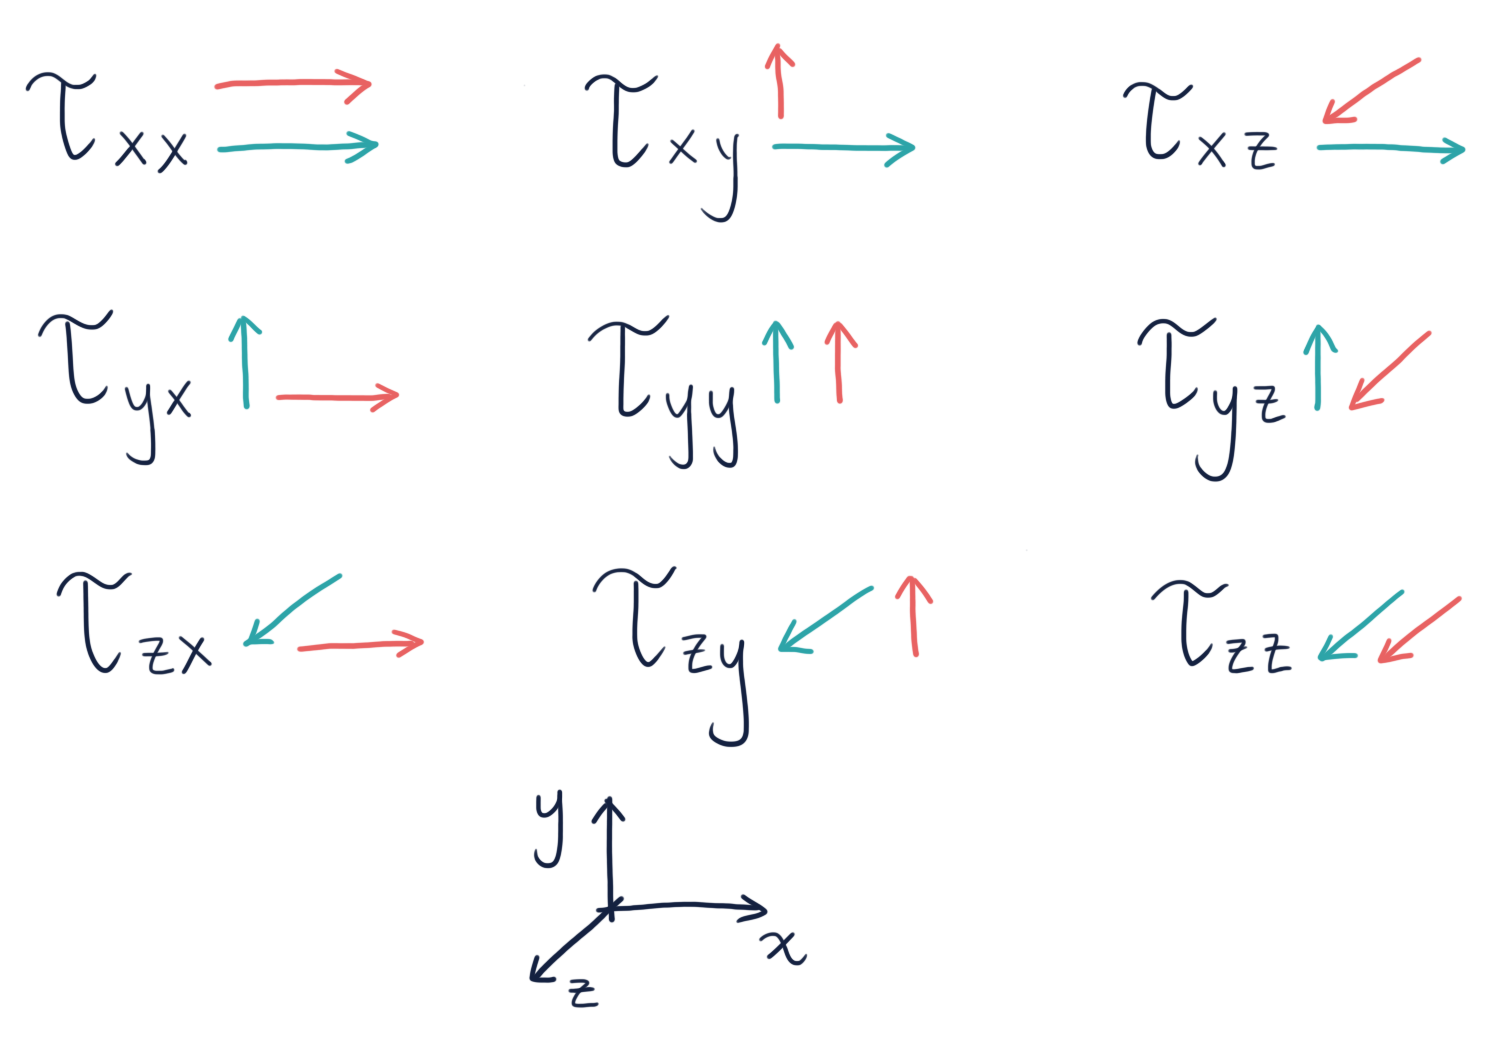
\includegraphics[width=8cm]{tensor-in-matrix-form.png}
\caption{Second-order tensor from the three-dimensional world. It can represent viscous momentum flux in a three-dimensional fluid flow.}
\label{fig:tensor-in-matrix-form}
\end{figure}

%\section*{Convective momentum flux tensor}

%Transport of a vector quantity is not the only application for a tensor. Another possibility could be keeping track of a vector quantity that is linked to a surface oriented in a particular direction (with the direction being defined by a unit normal vector). Imagine then having unit normal vectors in Cartesian coordinates $\hat{i}$, $\hat{j}$ and $\hat{k}$ that specify surfaces perpendicular to respectively $x$, $y$ and $z$ axis. At each of those surfaces 



% A flux of a vector quantity always requires the concept of a tensor!




%\section*{Operations on tensors}



\vspace{5mm}

%\section*{Epilogue}

%Some say that a good scientific writing that keeps the reader engaged is characterized by a single idea carried over from sentence to sentence that guides the reader through the journey. I hope that I managed to make this reading interesting to you by transporting the idea of a tensor downward this document!

%I wanted to use the momentum transport as a pretext to explain these bizzare objects that tensors are and I hope that I managed to make tensors the main character of this article. On the other hand, momentum transport in fluids has itself its peculiarities. Hopefully piggybacking the concept of a tensor was an overall useful experience for you!
















\thebibliography{}

\bibitem{BSL} R.B. Bird, W.E.Stewart, E.N. Lightfoot, \textit{Transport Phenomena}, John Wiley \& Sons, Inc., 2001

\end{document}